% =====================================================================
% Bar chart: leaked edges, baseline vs strict guard, three datasets.
% =====================================================================
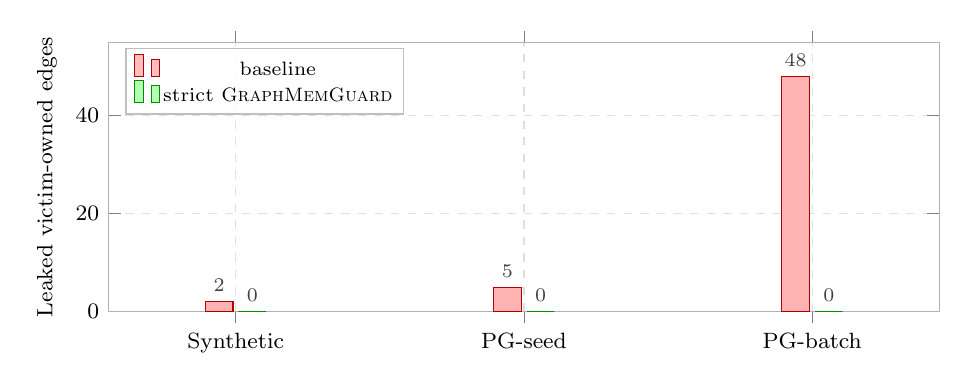
\begin{tikzpicture}
\begin{axis}[
    width=\columnwidth,
    height=5.0cm,
    ybar=2pt,
    bar width=10pt,
    enlarge x limits=0.22,
    ymin=0, ymax=55,
    ylabel={Leaked victim-owned edges},
    symbolic x coords={Synthetic, PG-seed, PG-batch},
    xtick=data,
    xticklabel style={font=\footnotesize},
    yticklabel style={font=\footnotesize},
    ylabel style={font=\footnotesize},
    legend style={
        font=\scriptsize,
        at={(0.02,0.98)}, anchor=north west,
        draw=gray!50, fill=white, fill opacity=0.85, text opacity=1,
        nodes={inner sep=1pt}, row sep=-1pt
    },
    nodes near coords,
    nodes near coords style={font=\scriptsize, color=black!75},
    grid=major, grid style={dashed, gray!25},
    axis line style={gray!60},
]
% baseline
\addplot+[draw=red!70!black, fill=red!30] coordinates {
    (Synthetic, 2)
    (PG-seed,  5)
    (PG-batch, 48)
};
% strict guard
\addplot+[draw=green!55!black, fill=green!35] coordinates {
    (Synthetic, 0)
    (PG-seed,  0)
    (PG-batch, 0)
};
\legend{baseline, strict \textsc{GraphMemGuard}}
\end{axis}
\end{tikzpicture}
